%% Figure from MATH 556 notes, section 43 (Lecture 18). ADDED (not from lecture).
\begin{tikzpicture}[>=stealth]
  \begin{scope}[xshift=0cm]
    \draw[->] (0,0) -- (3.6,0) node[right, font=\scriptsize] {$j$}; \draw[->] (0,0) -- (0,2.25);
    \draw[gray, dotted] (0,2) -- (3.4,2); \node[left, font=\scriptsize] at (0,2) {$1$};
    \fill[blue!60!black] (0.13,0) rectangle (0.27,2.000);
    \node[font=\small] at (1.7,2.65) {$N = 1$};
    \node[font=\scriptsize] at (1.7,-0.45) {$\bigl\| \tfrac1N (e_1 + \cdots + e_N) \bigr\| = 1$};
  \end{scope}
  \begin{scope}[xshift=4.6cm]
    \draw[->] (0,0) -- (3.6,0) node[right, font=\scriptsize] {$j$}; \draw[->] (0,0) -- (0,2.25);
    \draw[gray, dotted] (0,2) -- (3.4,2); \node[left, font=\scriptsize] at (0,2) {$1$};
    \fill[blue!60!black] (0.13,0) rectangle (0.27,0.500);
    \fill[blue!60!black] (0.33,0) rectangle (0.47,0.500);
    \fill[blue!60!black] (0.53,0) rectangle (0.67,0.500);
    \fill[blue!60!black] (0.73,0) rectangle (0.87,0.500);
    \node[font=\small] at (1.7,2.65) {$N = 4$};
    \node[font=\scriptsize] at (1.7,-0.45) {$\bigl\| \tfrac1N (e_1 + \cdots + e_N) \bigr\| = \tfrac12$};
  \end{scope}
  \begin{scope}[xshift=9.2cm]
    \draw[->] (0,0) -- (3.6,0) node[right, font=\scriptsize] {$j$}; \draw[->] (0,0) -- (0,2.25);
    \draw[gray, dotted] (0,2) -- (3.4,2); \node[left, font=\scriptsize] at (0,2) {$1$};
    \fill[blue!60!black] (0.13,0) rectangle (0.27,0.125);
    \fill[blue!60!black] (0.33,0) rectangle (0.47,0.125);
    \fill[blue!60!black] (0.53,0) rectangle (0.67,0.125);
    \fill[blue!60!black] (0.73,0) rectangle (0.87,0.125);
    \fill[blue!60!black] (0.93,0) rectangle (1.07,0.125);
    \fill[blue!60!black] (1.13,0) rectangle (1.27,0.125);
    \fill[blue!60!black] (1.33,0) rectangle (1.47,0.125);
    \fill[blue!60!black] (1.53,0) rectangle (1.67,0.125);
    \fill[blue!60!black] (1.73,0) rectangle (1.87,0.125);
    \fill[blue!60!black] (1.93,0) rectangle (2.07,0.125);
    \fill[blue!60!black] (2.13,0) rectangle (2.27,0.125);
    \fill[blue!60!black] (2.33,0) rectangle (2.47,0.125);
    \fill[blue!60!black] (2.53,0) rectangle (2.67,0.125);
    \fill[blue!60!black] (2.73,0) rectangle (2.87,0.125);
    \fill[blue!60!black] (2.93,0) rectangle (3.07,0.125);
    \fill[blue!60!black] (3.13,0) rectangle (3.27,0.125);
    \node[font=\small] at (1.7,2.65) {$N = 16$};
    \node[font=\scriptsize] at (1.7,-0.45) {$\bigl\| \tfrac1N (e_1 + \cdots + e_N) \bigr\| = \tfrac14$};
  \end{scope}
\end{tikzpicture}
